\documentclass[12pt]{article}
\usepackage{../../includes/assignment}
\usepackage{../../includes/math}
\usepackage{../../includes/uark_colors}

\newcommand{\answer}[1]{{\color{blue_winged_teal}\textbf{Answer:} #1}}
\newcommand{\pts}[1]{{\color{zinc500}(#1 pts)}}

\begin{document}
\begin{center}
  {\Huge\bf Final - Spring 2026}

  \smallskip
  {\large\it ECON 5753 — University of Arkansas}
\end{center}

\vspace{5mm}
\begin{enumerate}
  \item You are an analyst at a bike-share company in a major city. You have hourly bike rental data for the past 5 years and want to understand patterns in hourly rentals to forecast future demand.
    \begin{enumerate}
      \item \pts{10} List three types of time-series variables (functions of $t$) you would include in a time-series regression for hourly bike rentals and explain what time-series behavior each term captures.

      \answer{
        Examples include: 

        Seasonal patterns:
        \begin{itemize}
          \item Hour of day indicators to estimate patterns over the course of the day
          
          \item Day of week indicators to estimate patterns over the week
          
          \item Week of the year indicators or monthly indicators to estimate patterns over the year
          
          \item Fourier series to flexibly estimate seasonal patterns
        \end{itemize}

        Holiday effets:
        \begin{itemize}
          \item Indicators for holidays
        \end{itemize}

        Time trends:
        \begin{itemize}
          \item Linear time trend or piecewise linear trends
        \end{itemize}
      }

      \item \pts{10} Suppose the company launched a marketing campaign for the month of January 2024.
        How could you modify the regression to statistically test whether the campaign led to a statistically significant increase in rentals.
        Describe what you would look at in the regression output to test this hypothesis.

      \answer{
        Add an indicator variable for the month of January 2024.
        Look at the coefficient on that variable and test whether that coefficient is significantly different from 0.
      }

      \item \pts{10} Suppose you add hourly temperature (in degrees Fahrenheit) to the regression along with your other terms. Explain what the coefficient on temperature represents.
        Why might assuming a linear relationship be problematic?
        What could you do to address this?

      \answer{
        The coefficient would represent the marginal predictive effect comparing days with higher temperatures holding fixed the other time-series behavior included as control varaibles.
        The relationship between temperature and bike riding is probably non-linear with ridership peaking on `perfect days' and going down on very cold days and very hot days. 
        To addres this, I could either (i) use polynomials of temperature or (ii) create indicator for temperature bins!
      }

      \item \pts{5} Your manager asks you to report a forecast for next month's bike rentals.
        They say ``just give me a number so I know what to expect.''
        Why is it important to present a confidence interval (or range) rather than just a single point estimate when reporting this forecast?

      \answer{
        A point forecast gives only the most likely value, but it hides uncertainty around our estimate (e.g. sampling uncertainty).
        A confidence interval shows a range of plausible outcomes, which is what decision-makers need for planning risk (e.g., staffing, bike availability, and budget).
        If the interval is wide, that signals low precision of the estimate and suggests the manager should be less confident in the estimate.
      }

      \item \pts{5} Suppose another analyst suggests using a complex machine learning model with 20+ interactions that yields a slightly better in-sample fit.
        Give an example of when you would want to use the simpler regression model and an example where you would prefer the more complex model.

      \answer{
        The complex machine learning model might perform better at predicting ridership on a given day.
        However, the model would be hard to interpret and would be a `black box'. 
        The more simple linear regression is more useful for understanding relationships between certain variables and ridership (e.g. developing `heuristics').
      }
    \end{enumerate}

    \newpage
    \vspace*{2\bigskipamount}
  \item Say you have a sample of stores where you observe the average daily revenue and the number of employees on the sales floor.
    You regress the average daily revenue on the number of employees and estimate a coefficient of $\hat{\beta}_1 = 2247$ and a standard error of $\text{SE}(\hat{\beta}_1) = 980$.
    \begin{enumerate}
      \item \pts{5} Describe the thought experiment we discussed in class that generates the sampling distribution of $\hat{\beta}_1$ in the regression of average daily revenue on number of employees.
      
      \answer{
        The thought experiment is that of \emph{repeated sampling}.
        That is, drawing many different random samples of stores and rerunning the same regression for each sample. 
        The distribution of estimated coefficients would represent the sample distribution of the statistic.
      }

      \item \pts{10} The company does not want to increase the number of staff if these results are not statistically significant. Perform and report a test of the null that $\beta_1 = 0$ using a level of significance of $\alpha = 0.05$.
      
      \answer{
        In this case, the $t$-statistic is $(2247 - 0) / 980 = 2.29$.
        Since this statistic is larger than 1.96, we will reject the null that the population regression coefficient is $\beta_1 = 0$ with a 5\% level of significance.
      }

      \item \pts{10} Should this estimate be viewed as the causal effect of adding staff on the volume of sales? Why or why not?
      
      \answer{
        This should not be viewed as the causal estimate of adding staff because there are many potential missing variables that correlate with the number of staff. 
        For example, the store might put on extra staff on the weekends or during special sales events. 
        These days would have higher revenue and the extra staff will be `given credit' for these alternative causes.
      }
    \end{enumerate}

    \bigskip
  \item On the following pages, I present time-series data on monthly mortgage originations (in billions of dollars).
    Figure~\ref{fig:raw_ts} shows the raw data along with fitted values from a time-series regression.
    The time-series regression includes month-of-year indicators and a piecewise linear function of the \texttt{date} variable. 
    There are break points in the trend on January 1st of 2000, 2004, and 2009.
    Figure~\ref{fig:raw_ses} shows the raw data along with two SES (Simple Exponential Smoothing) smoothed series with different smoothing parameters.

    \begin{enumerate}
      \item \pts{5} Looking at Figure~\ref{fig:raw_ts}, suppose you wanted to test whether there is a statistically significant break in trend around 2009.
        What coefficient would you examine in the regression output and what is the result of that test? 

      \answer{
        The coefficient on \texttt{trend\_4} represents the change in slope from the previous epoch. 
        Since this coefficient is significantly different from zero ($^{***}$) we reject the null that there is no trend break around 2009. 
      }
        
      \item \pts{10} What is the estimated slope of the trend line starting in 2009?

      \answer{
        The slope is given by the sum of the trends coefficients up until the 2009 break:
        $$
          0.04 + 0.09 - 0.21 + 0.08 = 0.
        $$
      }

      \item \pts{5} Which month has the highest relative difference in mortgage originations? How do you know?

      \answer{June has the highest relative difference in mortgage originations. We know that because its coefficient is positive (higher than the omitted group January) and it is the largest in magnitude.}

      \item \pts{10} In Figure~\ref{fig:raw_ses}, compare the two SES smoothed lines. Which value of $\alpha_1$ or $\alpha_2$ is larger?
        How can you tell from this figure?

        \answer{$\alpha_1$ is higher because that line more closely follows period-specific shocks.}

      \item \pts{5} Say I was concerned that mortgage originations are correlated with the federal interest rate which I observe in my dataset. Which method, smoothing or regression, would be better to use for this?

      \answer{A time-series regression would be better in this case since I could include the federal interest rate as a control variable directly.}
    \end{enumerate}

    \newpage

    \begin{figure}[h!]
      \caption{Monthly Mortgage Originations: Raw Data + TS Regression}
      \label{fig:raw_ts}

      \vspace*{-2\bigskipamount}
      \begin{center}
        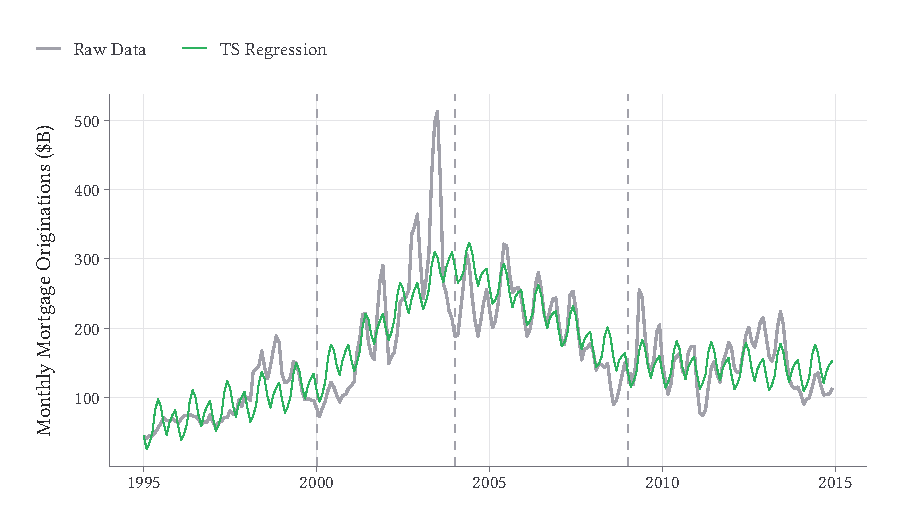
\includegraphics[width = 0.8\textwidth]{figures/raw_data_ts_regression.pdf}
      \end{center}
    \end{figure}

    \begin{figure}[h!]
      \caption{Monthly Mortgage Originations: Raw Data + SES Smoothing}
      \label{fig:raw_ses}

      \vspace*{-2\bigskipamount}
      \begin{center}
        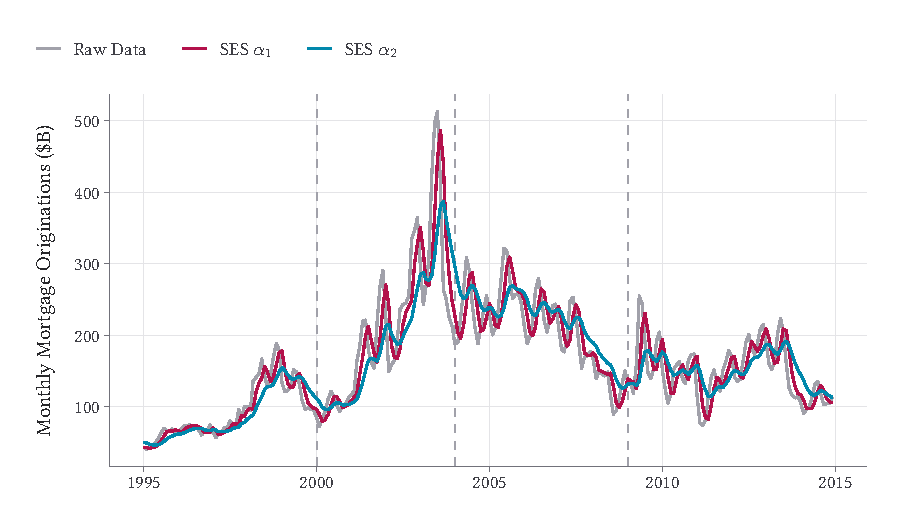
\includegraphics[width = 0.8\textwidth]{figures/raw_data_ses.pdf}
      \end{center}
    \end{figure}

    \newpage
    \begin{codeblock}[{}]
Dependent Var.: m_originations_billion

Constant              -286.0*** (58.9)
date                   0.04*** (0.006)
trend_2                 0.09*** (0.01)
trend_3                -0.21*** (0.02)
trend_4                 0.08*** (0.01)
month = Feb              -20.4. (10.7)
month = Mar               -13.0 (10.5)
month = Apr                0.68 (10.4)
month = May               32.8* (13.5)
month = Jun              47.4** (15.2)
month = Jul               35.8* (15.6)
month = Aug                 9.6 (12.5)
month = Sep                -7.5 (10.7)
month = Oct                 9.9 (11.9)
month = Nov                19.2 (13.3)
month = Dec               24.9. (13.6)
_______________ ______________________
S.E. type             Newey-West (L=0)
---
Signif. codes: 0 '***' 0.001 '**' 0.01 '*' 0.05 '.' 0.1 ' ' 1
    \end{codeblock}

\end{enumerate}
\end{document}
